\documentclass{article}
\usepackage{cancel}
\usepackage[utf8]{inputenc}
\usepackage[english,russian]{babel}
\usepackage{graphicx}
\graphicspath{{pictures/}}
\usepackage{amsmath}

\begin{document}

\begin{center}
	\subsection*{Задача 1}
\end{center}

Пусть люди - вершины графа $ G = (V, E) $, а ребро между ними - признак знакомства.
посмотрим на какое-либо ребро $ (u, v) \in E, \space u, v \in V $. По условию $ |N(u) \cap N(v)| = 5$.

Поймем, что $ (u, v) $ входит ровно в 5-ть троек попарно знакомых людей.

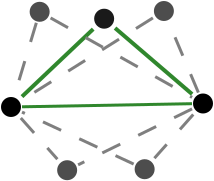
\includegraphics[scale=0.5]{1_1.png}

(Действительно, у двух знакомых людей ровно пять общих знакомых)
Тогда выразим кол-во таких троек попарно соед. вершин через число ребер: каждое ребро состоит в 5 треугольниках, тогда $|E| \cdot 5$ - число троек с повторами - каждый "треугольник" был посчитан ровно три раза, т.к. он был учтен для каждого из трех ребер "треугольника" $\Rightarrow$ всего троек:
$$ \frac{|E| \cdot 5}{3}$$

Но тогда, так как количество троек чисел может быть только целым, то число ребер кратно 3, т.к. 5 и 3 - взаимно просты. $ \Rightarrow $ число пар знакомых кратно 3.   
 
 \begin{center}
 	\subsection*{Задача 2}
 \end{center}
 
 \textbf{A)} $ n $ вершин. $ |E|_{max} = \frac{n(n - 1)}{2} $ - случай полного графа.
 $ |E|_{min} = n - 1 $. Докажем, что меньше быть не может.
 Возьмем какой-то связанный граф с $ n $ вершинами. Итеративно будем удалять из графа ребра, которые входят в какой-нибудь цикл, до тех пор, пока не останется граф $ G' = (V, E') $ без циклов. Поймем, что граф после этого останется связанным и докажем это в Задаче 5.
 
 Поймем, что в $ G' $ ровно $n - 1$ ребро и что больше нельзя удалить ребро не потеряв связанности. 
 Для начала докажем второе утв.: предположим, что можно удалить еще одно ребро $(u, v) \in E'$, не потеряв связанность, тогда $ \forall w \in V \exists $ простой путь из  $w$ в $u, v$, не проходящий через ребро $(u, v)$, но тогда существует и путь в $u$ проходящий через $(u, v)$  $ \Rightarrow $ в вершины $u, v$ можно добраться более чем одним путем, а это значит, что в графе есть какой-нибудь цикл, что не возможно по построению $ G' $.
 
 Докажем теперь, что $|E'| = n - 1$.  Возьмем какую-либо вершину степени 1 (ее существование будет доказано в задаче 5), удалим ее и ребро, из нее выходящее, получим связанный граф без циклов (показано в задаче 5), повторим до тех пор, пока не останется одна вершина. Всего мы удалим $ n - 1 $ вершину, а значит и $n - 1$ ребро, а т.к. больше ребер не осталось и на каждом шаге мы удаляли по 1-ой вершине, то ребер было $ n - 1 $.  
 
 Тогда в любом связанном графе есть подграф $G'=(V, E') \subset G = (V, E), |V| = n, |E'| = n - 1$. Значит в графе $ G $ хотя бы $ n - 1$ ребро.
 
\textbf{B)} Пусть $|V|$ - количество вершин, тогда пользуясь пунктом \textbf{А}:
\begin{equation*}
	\begin{cases}
		|V| - 1 <= n, \\
		\frac{|V|(|V| - 1)}{2} >= n 
	\end{cases}
\end{equation*}
$$ \Updownarrow $$
\begin{equation*}
	\begin{cases}
		|V| <= n + 1 \\
		\left[\begin{array}{l} 
			|V| >= \frac{1 + 2\sqrt{n}}{2}, \\ 
			|V| <= \frac{1 - 2\sqrt{n}}{2}. \end{array}\right. 
	\end{cases}
\end{equation*}

При $n = 0$, $|V| = 1$ или $|V| = 0$, иначе: 

\begin{equation*}
\begin{cases}
|V| - 1 <= n, \\
|V| > \lfloor\frac{1 + 2\sqrt{n}}{2}\rfloor
\end{cases}
\end{equation*}


\begin{center}
	\subsection*{Задача 3}
\end{center}

\textbf{A)} Нет. Например следующий граф из 4-х вершин не содержит цикла длины 3:
$|V| = 4$, степени вершин $(2;2;2;2)$

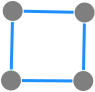
\includegraphics[scale=0.5]{3_1.png}

\textbf{B)} Да, обязательно есть. Докажем от противного: нет такого графа $ G = (V, E) $ с циклом длины 4, в котором $ |V| = 2n, \space \all u \in V: d(u) >= n,\space n >= 2 $ (иначе задача теряет смысл).

Разберем несколько случаев:

\textbf{I} 
$n \cancel{=} 2$ и В графе есть цикл длины 3 из вершин $ u, v, w \in V$. По предположению ни у каких двух вершин из $\{u, v, w\}$ нет общего соседа отличного от $\{u, v, w\}$, иначе существует цикл длины 4:

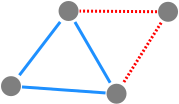
\includegraphics[scale=0.5]{3_2.png}

Значит сумма соседей $u,v,w$, отличных от $u,v,w$, и самих $u,v,w$ дают все вершины графа, т.к. множества соседей попарно не пересекается кроме как в вершинах из $\{u, v, w\}$. Но у каждой из вершин $\{u, v, w\}$ хотя бы $n - 2$ соседа отличных от $\{u, v, w\}$ (по условию, степень каждой вершины хотя бы $n$). Но значит в этом графе $N(u) + N(v) + N(w) - |{u}| - |{v}| - |{w}| <= |V| \Rightarrow 3n - 3 <= |V| <= 2n \Rightarrow n <= 3$
Значит $n = 3$. Тогда граф имеет вид хотя бы:

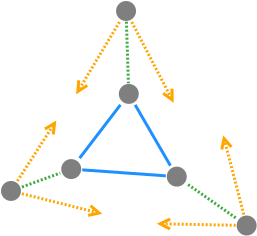
\includegraphics[scale=0.5]{3_3.png}
 
 Тогда например сосед $u$ соединен с кем-то из соседей $v, w$, и не соединен с $v, w$ (иначе он их общий сосед отличный от вершин цикла $\{u, v, w\}$ и есть цикл длины 4), но тогда эта пара соседей и 2-е вершины из цикла образуют цикл длины 4, что невозможно по предположению. 

\textbf{II}

Цикла длины 3 нет. Посмотрим на ребро $(u, v) \in E$. Тогда у $u, v \in V$ нет общих соседей. Это  возможно, только если у них ровно по $ n - 1 $ соседу. Посмотрим на $t \in N(u)$. Поймем, что $t$ соединен с кем-то из соседей $v$, т.к. циклов длины 3 нет, то $t$ не соединен с соседями $u$, и с вершиной $v$, значит единственная возможность - быть соединенным с соседями $v$. Но тогда посмотрим на ${t, x, u, v}$, где $x$ - общий сосед $t$ и $v$: эти вершины образуют цикл длины 4.
 
\textbf{III}

Цикл длины 3 есть, $n = 2$. Все возможные такие графы: полный и полный без одного ребра. (выделим цикл, у вершины вне этого цикла две возможные степени: $2$ - полный без ребра и $3$ - полный граф). Но в этих графах есть и цикл длины 4:

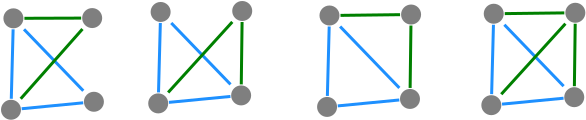
\includegraphics[scale=0.5]{3_5.png}

Тогда в любом таком графе есть цикл длины 4.
 \\
 
\begin{center}
	\subsection*{Задача 5}
\end{center}
Пусть $ G = (V, E) $. 
Если граф содержит какие-нибудь циклы, тогда возьмем цикл $ \{u_0, u_1, ... u_n\},\space u_i \in V$. Поймем, что из него можно выкинуть какое-либо ребро, не повредив связанности графа (Действительно, если есть какой-нибудь путь из $v $ в $w$, проходящий через ребро $ (u_k, u_m) $, то существует путь проходящий через прочие ребра цикла, ведь в цикле до каждой вершины можно дойти хотя бы двумя разными путями $\Rightarrow$ граф без этого ребра останется связанным). Тогда выкинем его. Повторим до тех пор пока в графе не останется циклов. 

Имеем $ G' \subseteq G,\space V' = V $. 
Докажем, что в $ G' $ есть вершина степени $ 1 $.
Возьмем, какую либо вершину этого графа. Перейдем в ее соседа, если у соседа нет ребер, отличных от того, по которому мы в него пришли, остановимся в соседе, иначе: перейдем по этому отличному ребру, в еще не посещенную вершину. Будем повторять эти переходы. Поймем, что раз граф связан и количество вершин конечно, то рано или поздно мы не сможем перейти. Это возможно в двух случаях: либо мы оказались в вершине со степенью 1, либо мы не можем перейти в посещенную вершину, что означает наличие цикла, а значит недостижимо. Значит мы остановились в вершине со степенью 1$\Rightarrow$ она существует.

Тога эту вершину можно удалить, не навредив связанности графа, т.к. любой простой путь проходящий по ее ребру ведет в эту вершину или из нее, т.е. только соединяет эту вершину с оставшимися, тогда в отсутствии этой вершины исчезнут только те пути, что вели в нее, а значит граф по прежнему останется связанным.

Тогда эту же вершину можно удалить и из начального графа $G$, не вредя связанности, т.к. в нем есть связанный $G''$ (граф без вершины степени из $G'$). 
\begin{center}
	\subsection*{Задача 6}
\end{center}
Предположим противное: ни сам граф $ G = (V, E) $, ни его дополнение $ \bar{G} $ не содержат циклы длины $ 3 $.

Это означает, что в графе $ G $ нет таких 3-х вершим между которыми нет ни одного ребра и таких 3-х вершин, которые попарно соединены между собой.
Тогда любые 3 вершины в графе соединяются одним из двух способов.
\\
\\


\includegraphics[scale=0.5]{6_1.png} 


Т.е. в любой тройке людей есть либо два незнакомых человека, либо два знакомых. 

Поймем, что у какого-нибудь человека $u$ либо 3 и более знакомых \textbf{(1)}, либо 3 и более незнакомых \textbf{(2)}(т.к. всего людей хотя бы 6, по принципу Дирихле).

1) Среди трех знакомых с $u$ есть хотя бы два знакомых между собой (по предположению), значит с  $u$ они образуют цикл длины 3.
 
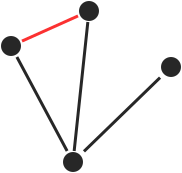
\includegraphics[scale=0.5]{6_2.png}

Что невозможно по предположению.

2) Среди трех незнакомых $u$ есть хотя бы два не знакомых между собой человека (т.к. они образуют тройку), а значит вместе с $u$ они образуют тройку попарно незнакомых.

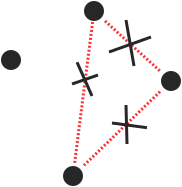
\includegraphics[scale=0.5]{6_3.png}

Но тогда эти три незнакомых в $\bar{G}$ образуют цикл длины 3.
Что не возможно по предположению.
Противоречие. $\Rightarrow$ Граф с более чем пятью вершинами или его дополнение содержат цикл длины 3.
\newpage
\\
\textbf{A)} В данном графе и его дополнении есть только цикл длины 5.

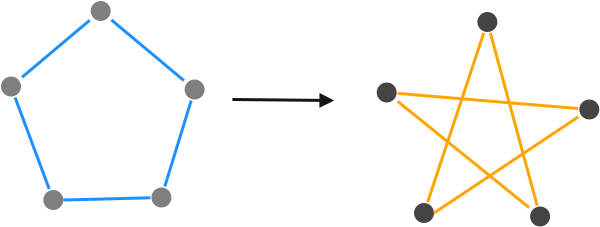
\includegraphics[scale=0.5]{6_4.png}

\textbf{B)} Примеры графов без циклов, дополнения которых так же не содержат циклы для $G = (V, E); |V| <= 4 $ (пунктир - ребра дополнения):


\includegraphics[scale=0.5]{6_5.png}

Докажем, что если $|V| = 5$, то $G$ содержит цикл.
Разберем случаи, когда граф связан и когда не связан.

\textbf{I} 

(1) Граф связан и в нем есть цикл - задача решена.

(2) Граф связан, цикла нет, тогда есть висячая вершина $u$ (см. 5). Тогда в дополнении $ \bar{G} $ $u$ соединена с тремя вершинами, с которыми не соединена в начальном графе. Но как мы помним в $G$ циклов нет $\Rightarrow$ хотя бы две вершины из этих трех не соединены между собой в $G$, а значит соединены в $\bar{G}$, а значит есть цикл длины 3 в дополнении из вершины $u$ и тех двух не соединенных в начальном графе.

\textbf{II} 

(1) Граф не связан и в нем есть цикл - задача решена.

(2) Граф не связан, циклов нет. Поймем, что если компонент связанности больше 2-х, то в дополнении все вершины из разных компонент соединены между собой, а значит есть цикл длины хотя бы 3. Если компонент - 2, то либо в одной 3 вершины а во второй 2, либо в одной 1 во второй 4.

В обоих случаях в больших компонентах есть хотя бы две не соединенных вершины (иначе есть цикл), между которыми есть ребро в дополнении, а вершины(а) из меньшей компоненты в дополнении соединена со всеми вершинами большей компоненты $\Rightarrow$ соединена с двумя соединенными вершинами $ \Rightarrow $ есть цикл. 	

\end{document}